\documentclass[handout, 11pt]{beamer}
\mode
<presentation>{\usetheme{Madrid}}
\institute[UF]{\inst{1}
University of Florida\\
Department of Finance, Insurance, and Real Estate}
\usepackage{adjustbox}
\usepackage{tikz}
\usetikzlibrary{positioning}
\usetikzlibrary{positioning}
\usetikzlibrary{positioning}
\usetikzlibrary{positioning}
\usetikzlibrary{positioning}
\usetikzlibrary{positioning}
\usetikzlibrary{positioning}
\usetikzlibrary{positioning}
\usetikzlibrary{positioning}
\usetikzlibrary{positioning}
\usetikzlibrary{positioning}
\usetikzlibrary{positioning}
\usetikzlibrary{positioning}
\usetikzlibrary{positioning}
\usetikzlibrary{positioning}
\usepackage{booktabs}
\definecolor{darkgreen}{RGB}{31,156,17}
\usepackage{minted}
\usepackage{xcolor}
\setbeamertemplate{headline}{\begin{beamercolorbox}[ht=2.25ex, dp=3.75ex]{section in head/foot}
\insertnavigation{\paperwidth}
\end{beamercolorbox}}
\AtBeginSection{\begin{frame}
\frametitle{Table of Contents}
\tableofcontents[currentsection]
\end{frame}}
\begin{document}
\title[Sensitivity Analysis]{Exploring the Parameter Space}
\subtitle{Pt. 1: Sensitivity Analysis}
\author[DeRobertis]{Nick DeRobertis\inst{1}}
\date{\today}
\begin{frame}
\titlepage
\label{title-frame}
\end{frame}
\begin{section}[Explore Parameters]{Introduction to Parameter Exploration}
\begin{frame}
\frametitle{Moving from a Static Model}
\begin{itemize}
\item So far, I have given you some inputs to use and you have been getting one or more outputs from those inputs
\vfill
\item We have not considered how those inputs may change, and how that affects the outputs
\vfill
\item This is where building a model vs. doing a calculation really starts to pay off
\end{itemize}
\end{frame}
\begin{frame}
\frametitle{How to Explore Inputs and their Affect on Outputs}
\begin{center}
\begin{adjustbox}{width=0.9\textwidth, height=0.8\textheight, keepaspectratio}
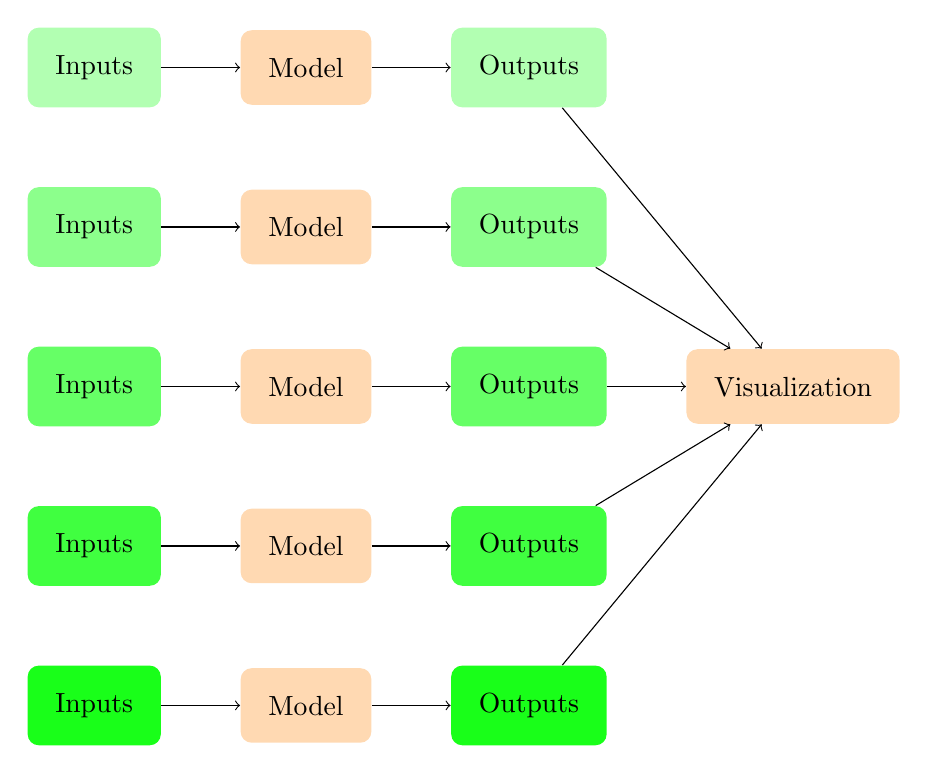
\begin{tikzpicture}
\node [fill=green!30, rounded corners, inner sep=10pt] (c76dabc2-1964-4a10-b72a-88fafa6f2138)  {Inputs};
\node [fill=orange!30, rounded corners, inner sep=10pt, right=of c76dabc2-1964-4a10-b72a-88fafa6f2138] (ab3d5dad-7dfb-43ae-aa5d-3acc752e0aad)  {Model};
\node [fill=green!30, rounded corners, inner sep=10pt, right=of ab3d5dad-7dfb-43ae-aa5d-3acc752e0aad] (f9bf7c24-76fd-46b5-aab1-e33305c3d589)  {Outputs};
\path [draw, ->] (c76dabc2-1964-4a10-b72a-88fafa6f2138) -- (ab3d5dad-7dfb-43ae-aa5d-3acc752e0aad);
\path [draw, ->] (ab3d5dad-7dfb-43ae-aa5d-3acc752e0aad) -- (f9bf7c24-76fd-46b5-aab1-e33305c3d589);
\node [fill=green!45, rounded corners, inner sep=10pt, below=of c76dabc2-1964-4a10-b72a-88fafa6f2138] (77b7cfc5-f237-4b8b-ade6-b2b41b402949)  {Inputs};
\node [fill=orange!30, rounded corners, inner sep=10pt, right=of 77b7cfc5-f237-4b8b-ade6-b2b41b402949] (170050d0-04a2-4a41-8a84-c7c58c1e31e8)  {Model};
\node [fill=green!45, rounded corners, inner sep=10pt, right=of 170050d0-04a2-4a41-8a84-c7c58c1e31e8] (4a6151fc-a83a-4b5b-9e7c-e5ffde1e4b60)  {Outputs};
\path [draw, ->] (77b7cfc5-f237-4b8b-ade6-b2b41b402949) -- (170050d0-04a2-4a41-8a84-c7c58c1e31e8);
\path [draw, ->] (170050d0-04a2-4a41-8a84-c7c58c1e31e8) -- (4a6151fc-a83a-4b5b-9e7c-e5ffde1e4b60);
\node [fill=green!60, rounded corners, inner sep=10pt, below=of 77b7cfc5-f237-4b8b-ade6-b2b41b402949] (755d7c98-4778-44f2-bbf4-030d2473a6b6)  {Inputs};
\node [fill=orange!30, rounded corners, inner sep=10pt, right=of 755d7c98-4778-44f2-bbf4-030d2473a6b6] (133a4ad1-cb06-49dc-9e20-34fbe122a1bf)  {Model};
\node [fill=green!60, rounded corners, inner sep=10pt, right=of 133a4ad1-cb06-49dc-9e20-34fbe122a1bf] (80db54e7-5856-4ac2-83b1-7aaf33e6df66)  {Outputs};
\path [draw, ->] (755d7c98-4778-44f2-bbf4-030d2473a6b6) -- (133a4ad1-cb06-49dc-9e20-34fbe122a1bf);
\path [draw, ->] (133a4ad1-cb06-49dc-9e20-34fbe122a1bf) -- (80db54e7-5856-4ac2-83b1-7aaf33e6df66);
\node [fill=green!75, rounded corners, inner sep=10pt, below=of 755d7c98-4778-44f2-bbf4-030d2473a6b6] (c112de39-eed3-4d4d-a44c-c4ed6acd5201)  {Inputs};
\node [fill=orange!30, rounded corners, inner sep=10pt, right=of c112de39-eed3-4d4d-a44c-c4ed6acd5201] (8fe197b4-2a19-4c68-b29d-77606584eb06)  {Model};
\node [fill=green!75, rounded corners, inner sep=10pt, right=of 8fe197b4-2a19-4c68-b29d-77606584eb06] (fc4cf0e5-0c0b-4c33-b31a-5733e1241913)  {Outputs};
\path [draw, ->] (c112de39-eed3-4d4d-a44c-c4ed6acd5201) -- (8fe197b4-2a19-4c68-b29d-77606584eb06);
\path [draw, ->] (8fe197b4-2a19-4c68-b29d-77606584eb06) -- (fc4cf0e5-0c0b-4c33-b31a-5733e1241913);
\node [fill=green!90, rounded corners, inner sep=10pt, below=of c112de39-eed3-4d4d-a44c-c4ed6acd5201] (228c44fd-358e-471a-ba35-a10d2827c4bf)  {Inputs};
\node [fill=orange!30, rounded corners, inner sep=10pt, right=of 228c44fd-358e-471a-ba35-a10d2827c4bf] (ec5d97db-2b15-4d47-b739-37459c049e05)  {Model};
\node [fill=green!90, rounded corners, inner sep=10pt, right=of ec5d97db-2b15-4d47-b739-37459c049e05] (3cc024c3-c59c-4785-b03b-7a2ac843d684)  {Outputs};
\path [draw, ->] (228c44fd-358e-471a-ba35-a10d2827c4bf) -- (ec5d97db-2b15-4d47-b739-37459c049e05);
\path [draw, ->] (ec5d97db-2b15-4d47-b739-37459c049e05) -- (3cc024c3-c59c-4785-b03b-7a2ac843d684);
\node [fill=orange!30, rounded corners, inner sep=10pt, right=of 80db54e7-5856-4ac2-83b1-7aaf33e6df66] (68b4c6ee-00a7-40d9-88fe-fb75febf9b0f)  {Visualization};
\path [draw, ->] (f9bf7c24-76fd-46b5-aab1-e33305c3d589) -- (68b4c6ee-00a7-40d9-88fe-fb75febf9b0f);
\path [draw, ->] (4a6151fc-a83a-4b5b-9e7c-e5ffde1e4b60) -- (68b4c6ee-00a7-40d9-88fe-fb75febf9b0f);
\path [draw, ->] (80db54e7-5856-4ac2-83b1-7aaf33e6df66) -- (68b4c6ee-00a7-40d9-88fe-fb75febf9b0f);
\path [draw, ->] (fc4cf0e5-0c0b-4c33-b31a-5733e1241913) -- (68b4c6ee-00a7-40d9-88fe-fb75febf9b0f);
\path [draw, ->] (3cc024c3-c59c-4785-b03b-7a2ac843d684) -- (68b4c6ee-00a7-40d9-88fe-fb75febf9b0f);
\end{tikzpicture}
\end{adjustbox}
\end{center}
\end{frame}
\begin{frame}
\frametitle{Methods of Parameter Exploration}
\begin{itemize}
\item In this lecture, we will be discussing sensitivity analysis as an approach to exploring the parameter space.
\vfill
\item After we cover probabilistic modeling, we will revisit exploring the parameter space with a method called Monte Carlo Simulation.
\vfill
\item In sensitivity analysis, a fixed set of values for the parameters are chosen, while in Monte Carlo Simulation, each parameter is assigned a distribution.
\vfill
\item Both methods may be used together to fully understand a model.
\end{itemize}
\end{frame}
\end{section}
\begin{section}[SA Theory]{Sensitivity Analysis Theory}
\begin{frame}
\frametitle{Sensitivity Analysis, Formally}
For the model given by:
\begin{equation}
	y = f(X)
\end{equation}
\begin{equation}
	X = [x_1, x_2, ..., x_n]
\end{equation}
\begin{itemize}
\item $y:$
Model output
\item $X:$
Model input matrix
\item $x_i:$
Value of $i$th $x$ variable
\end{itemize}
Follow the following steps:
\begin{enumerate}
\item Choose a set of values for each
$x_i$
\item Take the cartesian product of these values as
$[X_1, X_2, ..., X_m]$
\item For each
$X_i$
calculate
$y_i = f(X_i)$
\item Store the values of
$X_i$
mapped to
$y_i$
\item Visualize
$y_i$
versus
$X_i$
\end{enumerate}
\end{frame}
\begin{frame}
\frametitle{Sensitivity Analysis Example Model}
Let's take a simple demand model as an example:
\begin{equation}
	D = c - EP
\end{equation}
\begin{equation}
	X = [c, E, P]
\end{equation}
\begin{itemize}
\item $D:$
Quantity demanded
\item $c:$
Demand constant
\item $E:$
Elasticity of demand
\item $P:$
Price
\item $X:$
Model input matrix
\end{itemize}
\end{frame}
\begin{frame}
\frametitle{Sensitivity Analysis Example}
\begin{equation}
	D = c - EP
\end{equation}
Follow the following steps:
\begin{enumerate}
\item Choose
$c = (60000, 100000), E = (200, 500), P = (50, 100)$
\item Take the cartesian product of these values, yielding
$[X_1, X_2, ..., X_m]:$
\end{enumerate}
\begin{tabular}{ccc}
$c$ & $E$ & $P$\\
  60000 &  200 &   50 \\
  60000 &  200 &  100 \\
  60000 &  500 &   50 \\
  60000 &  500 &  100 \\
 100000 &  200 &   50 \\
 100000 &  200 &  100 \\
 100000 &  500 &   50 \\
 100000 &  500 &  100 \\

\end{tabular}
\end{frame}
\begin{frame}
\frametitle{Sensitivity Analysis Example, Pt. 2}
\begin{equation}
	D = c - EP
\end{equation}
Continue following the steps:
\begin{enumerate}
\setcounter{enumi}{2}
\item For each
$X_i$
calculate
$y_i = f(X_i)$
\item Store the values of
$X_i$
mapped to
$y_i$
\end{enumerate}
\begin{tabular}{cccc}
$c$ & $E$ & $P$ & $D$\\
  60000 &  200 &   50 &  50000 \\
  60000 &  200 &  100 &  40000 \\
  60000 &  500 &   50 &  35000 \\
  60000 &  500 &  100 &  10000 \\
 100000 &  200 &   50 &  90000 \\
 100000 &  200 &  100 &  80000 \\
 100000 &  500 &   50 &  75000 \\
 100000 &  500 &  100 &  50000 \\

\end{tabular}
\end{frame}
\end{section}
\begin{section}[SA Excel]{Sensitivity Analysis in Excel with Data Tables}
\begin{frame}
\frametitle{Sensitivity Analysis in Excel}
\begin{center}
\begin{adjustbox}{width=0.9\textwidth, height=0.8\textheight, keepaspectratio}
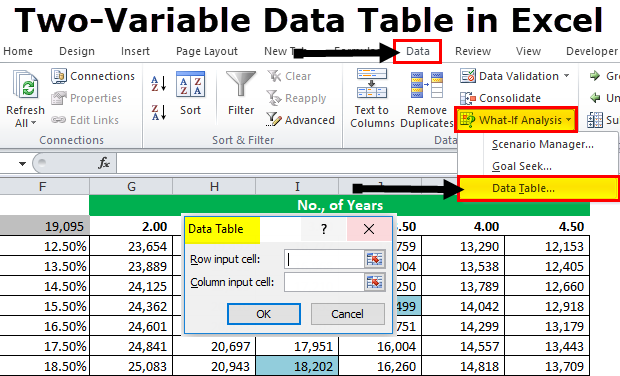
\includegraphics[width=1.0\textwidth]{Sources/excel-data-table.png}
\end{adjustbox}
\end{center}
\end{frame}
\begin{frame}
\frametitle{Visualizing Sensitivity Analysis in Excel}
\begin{itemize}
\item There are two main ways to visualize sensitivity analysis results in Excel: graphing and conditional formatting.
\vfill
\item Graphing is usually appropriate for one-way data tables
\vfill
\item Conditional formatting is usually appropriate for two-way data tables
\end{itemize}
\end{frame}
\begin{frame}
\frametitle{Conditional Formatting in Excel}
\begin{center}
\begin{adjustbox}{width=0.9\textwidth, height=0.8\textheight, keepaspectratio}
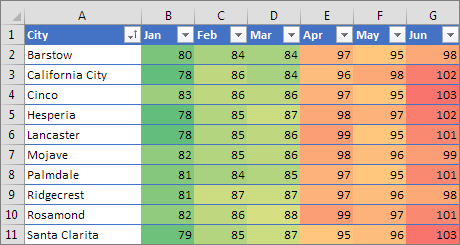
\includegraphics[width=1.0\textwidth]{Sources/excel-conditional-formatting.png}
\end{adjustbox}
\end{center}
\end{frame}
\begin{frame}
\frametitle{Sensitivity Analysis in Excel}
{
\setbeamercolor{block title}{bg=darkgreen}
\begin{block}{Adding Sensitivity Analysis to the Dynamic Retirement Excel Model}
\begin{itemize}
\item I will now go through adding sensitivity analysis to the Dynamic Salary Retirement Model in Excel
\item The completed exercise is in Examples > Sensitivity Analysis > Excel > Dynamic Salary Retirement Model Sensitivity.xlsx
\end{itemize}
\end{block}
}
\end{frame}
\begin{frame}
\frametitle{Sensitivity Analysis in Excel Lab}
{
\setbeamercolor{block title}{bg=violet}
\begin{block}{Adding Sensitivity Analysis to Project 1 - Excel}
\begin{enumerate}
\item Add sensitivity analysis to your Excel model from Project 1
\item See how the NPV changes when the number of machines and initial demand change
\item Do a one-way Data Table with a graph for each of the two inputs, then a two-way data table with conditional formatting
\end{enumerate}
\vfill
\begin{tabular*}{\textwidth}{@{\extracolsep{\fill}}ccc}
\toprule
\hfill & Resources: Slide \textcolor{blue}{\underline{\ref{labs:sensitivity-analysis-in-excel-lab-1-resources}}} & \hfill\\

\end{tabular*}
\end{block}
}
\label{labs:sensitivity-analysis-in-excel-lab-1}
\end{frame}
\end{section}
\begin{section}[Extra Python Basics]{Python List Comprehensions, Installing Packages, and More on Dictionaries}
\begin{frame}
\frametitle{Going Deeper into Python Code Structure}
We'll cover a couple more Python patterns and a new data type before jumping into sensitivity analysis
\begin{itemize}
\item Dictionaries
\item List comprehensions
\item Python
\texttt{import}
system and custom code
\end{itemize}
\end{frame}
\begin{frame}
\frametitle{What is a Dictionary?}
\begin{columns}
\begin{column}{0.5\textwidth}
\vbox to 0.8\textheight{\begin{itemize}
\item A dictionary, or
\texttt{dict}
for short, is another basic Python data type like lists, numbers, and strings.
\vfill
\item Like a list, it is a collection: it holds other objects.
\vfill
\item Unlike a list, a
\texttt{dict}
is composed of key-value pairs. It holds relationships between objects.
\end{itemize}}
\end{column}
\begin{column}{0.5\textwidth}
\vbox to 0.8\textheight{\centering
\vfill
\begin{tikzpicture}
\node [anchor=south west] (e3ecad63-11ff-437b-bf47-b7a337066c1a)  {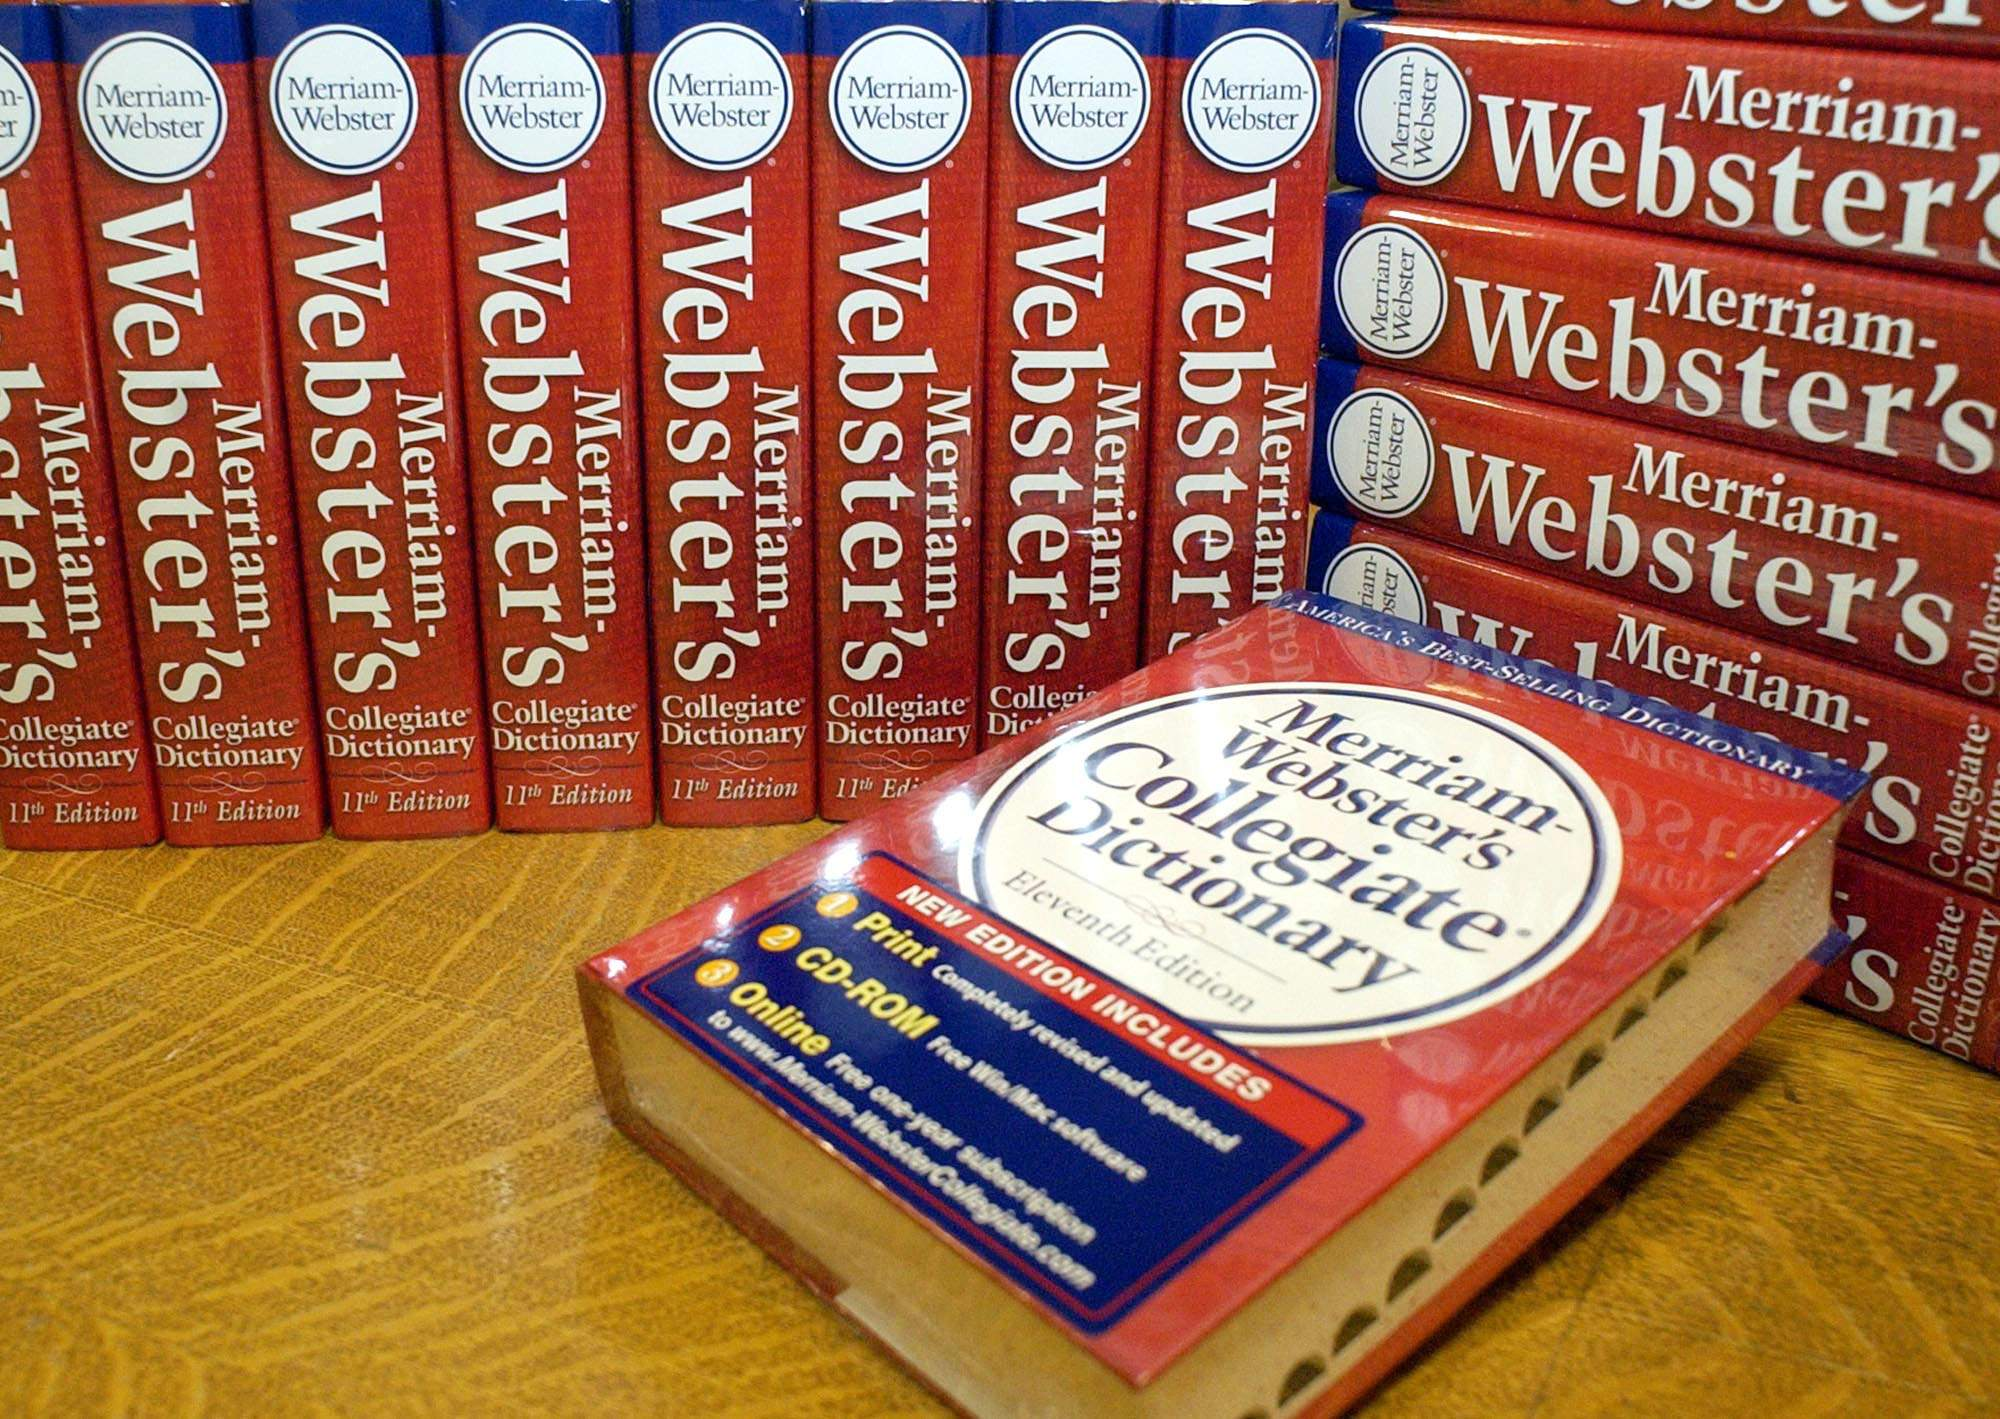
\includegraphics[width=1.0\textwidth]{Sources/dictionary-book.jpg}};
\begin{scope}[x={(e3ecad63-11ff-437b-bf47-b7a337066c1a.south east)}, y={(e3ecad63-11ff-437b-bf47-b7a337066c1a.north west)}]
\path [draw, radius=0.4, red, line width=5mm] (0.5, 0.5) circle;
\path [draw, red, line width=5mm] (0.2, 0.75) -- (0.8, 0.2);
\end{scope}
\end{tikzpicture}
\vfill
\vfill}
\end{column}
\end{columns}
\end{frame}
\begin{frame}[fragile]
\frametitle{How to Use Dictionaries}
\begin{block}{Basic Dictionary Example}
\footnotesize
\begin{minted}{python}

>>> coffee_levels_emotions = {
>>>     'high': 'happy',
>>>     'pretty high': 'happy',
>>>     'medium': 'neutral',
>>>     'low': 'sad',
>>>     'empty': 'desparate'
>>> }
>>> coffee_levels_emotions['pretty high']
'happy'
>>> for coffee_level, emotion in coffee_levels_emotions.items():
>>>     print(f"I'm {emotion} when my coffee is {coffee_level}")

\end{minted}
\texttt{I'm happy when my coffee is high}

\texttt{I'm happy when my coffee is pretty high}

\texttt{I'm neutral when my coffee is medium}

\texttt{I'm sad when my coffee is low}

\texttt{I'm desparate when my coffee is empty}

\texttt{    }

\end{block}
\end{frame}
\begin{frame}[fragile]
\frametitle{How to Modify Dictionaries}
\begin{block}{Add and Delete Items from Dictionaries}
\begin{minted}{python}

>>> coffee_levels_emotions.update({'overflowing': 'burned'})
>>> coffee_levels_emotions['negative'] = 'confused'
>>> high_value = coffee_levels_emotions.pop('high')
>>> coffee_levels_emotions
{'pretty high': 'happy',
 'medium': 'neutral',
 'low': 'sad',
 'empty': 'desparate',
 'overflowing': 'burned',
 'negative': 'confused'}
>>> high_value
'happy'

\end{minted}
\end{block}
\end{frame}
\begin{frame}
\frametitle{More About Dictionaries in Python}
{
\setbeamercolor{block title}{bg=darkgreen}
\begin{block}{Using Dictionaries}
\begin{itemize}
\item I will now start going through the example notebook in Examples > Sensitivity Analysis > Python > Python Dicts, List comprehensions, and Imports.ipynb
\item I will go through the Dictionaries section for now
\end{itemize}
\end{block}
}
\end{frame}
\begin{frame}
\frametitle{Dictionaries Lab}
{
\setbeamercolor{block title}{bg=violet}
\begin{block}{Learning How to Use Dictionaries}
\begin{enumerate}
\item For this Python section, lab exercises are in the Jupyter notebook Dicts and List Comprehensions Lab.ipynb
\item Complete the exercises in the dictionaries section for now
\end{enumerate}
\vfill
\begin{tabular*}{\textwidth}{@{\extracolsep{\fill}}ccc}
\toprule
\hfill & Resources: Slide \textcolor{blue}{\underline{\ref{labs:dictionaries-lab-1-resources}}} & \hfill\\

\end{tabular*}
\end{block}
}
\label{labs:dictionaries-lab-1}
\end{frame}
\begin{frame}[fragile]
\frametitle{An Easier way to Build Simple Lists from Loops}
\small
\begin{block}{The Original Way}
\begin{minted}{python}

>>> out_values = []
>>> for i in range(5):
>>>     out_values.append(i + 10)
>>> out_values
[10, 11, 12, 13, 14]

\end{minted}
\end{block}
\begin{block}{With List Comprehension}
\begin{minted}{python}

>>> out_values = [i + 10 for i in range(5)]
>>> out_values
[10, 11, 12, 13, 14]

\end{minted}
\end{block}
\begin{block}{Notice}
You
\textbf{never}
need to use list comprehension, it is just for convenience. The original
\texttt{for}
loop syntax will always work fine.
\end{block}
\end{frame}
\begin{frame}
\frametitle{Easier Loops in Python}
{
\setbeamercolor{block title}{bg=darkgreen}
\begin{block}{Using List Comprehensions}
\begin{itemize}
\item I will continue going through the example notebook in Examples > Sensitivity Analysis > Python > Python Dicts, List comprehensions, and Imports.ipynb
\item I will go through the List Comprehensions section for now
\end{itemize}
\end{block}
}
\end{frame}
\begin{frame}
\frametitle{List Comprehensions Lab}
{
\setbeamercolor{block title}{bg=violet}
\begin{block}{Learning How to Use List Comprehensions}
\begin{enumerate}
\item Continue working on the same Jupyter notebook from the previous lab exercise
\item Complete the exercises in the List Comprehensions section for now
\end{enumerate}
\vfill
\begin{tabular*}{\textwidth}{@{\extracolsep{\fill}}ccc}
\toprule
\hfill & Resources: Slide \textcolor{blue}{\underline{\ref{labs:list-comprehensions-lab-1-resources}}} & \hfill\\

\end{tabular*}
\end{block}
}
\label{labs:list-comprehensions-lab-1}
\end{frame}
\begin{frame}
\frametitle{Understanding Python \texttt{import}s}
\begin{itemize}
\item In the past we have used
\texttt{import}
to load packages such as
\texttt{numpy}
and
\texttt{pandas}
\vfill
\item These packages are just Python files. We can also write our own Python files and
\texttt{import}
them the same way
\vfill
\item When you \texttt{import something}, Python first searches the current directory for a file
\texttt{something.py}
and if it doesn't find it, it searches your installed packages
\vfill
\item In fact if you added a
\texttt{numpy.py}
in the current directory and tried to
\texttt{import}
\texttt{numpy}
it would
\texttt{import}
the contents of that file rather than the
\texttt{numpy}
package.
\end{itemize}
\end{frame}
\begin{frame}
\frametitle{Importing Custom Code}
\begin{itemize}
\item You can write your own functions and classes, then put them in a Python file and
\texttt{import}
them into your notebook.
\vfill
\item When you
\texttt{import}
a file, it executes the contents of that file. So you generally want just function and class definitions, and not really anything outside of
\texttt{def}
or
\texttt{class}
statements.
\vfill
\item Using Python files is a more maintainable structure for building complex models and apps versus Jupyter notebooks only.
\end{itemize}
\end{frame}
\begin{frame}
\frametitle{Installing Packages}
\begin{itemize}
\item Sometimes you will need a package which does not already come installed with Anaconda
\vfill
\item The general way to do this is with
\texttt{pip install mypackage}
replacing mypackage with
the package you want to install
\vfill
\item You would run this in Anaconda Prompt, or in Jupyter you can run it but you need to put an exclaimation mark before it to say you want to run it in a terminal. So in Jupyter it would be
\texttt{!pip install mypackage}
\end{itemize}
\end{frame}
\begin{frame}
\frametitle{Installing Packages in Python}
{
\setbeamercolor{block title}{bg=darkgreen}
\begin{block}{How to Install Packages}
\begin{itemize}
\item I will continue going through the example notebook in Examples > Sensitivity Analysis > Python > Python Dicts, List comprehensions, and Imports.ipynb
\item I will go through the Imports and Installing Packages section for now
\end{itemize}
\end{block}
}
\end{frame}
\end{section}
\begin{section}[SA Python]{Sensitivity Analysis in Python}
\begin{frame}
\frametitle{Sensitivity Analysis in Python - Hex-Bin}
\begin{center}
\begin{adjustbox}{width=0.9\textwidth, height=0.8\textheight, keepaspectratio}
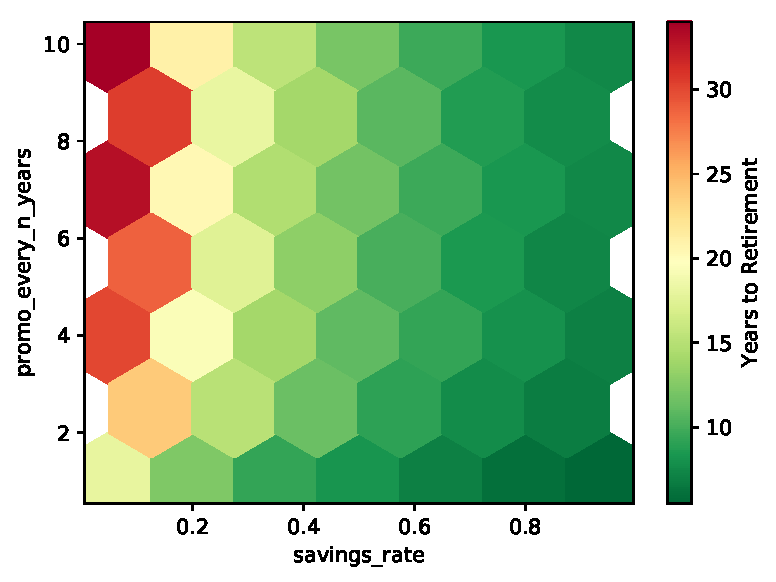
\includegraphics[width=1.0\textwidth]{Sources/python-sensitivity-hex-bins.pdf}
\end{adjustbox}
\end{center}
\end{frame}
\begin{frame}
\frametitle{Sensitivity Analysis in Python - Styled DataFrame}
\begin{center}
\begin{adjustbox}{width=0.9\textwidth, height=0.8\textheight, keepaspectratio}
\includegraphics[width=1.0\textwidth]{Sources/sensitivity-analysis-styled-df.png}
\end{adjustbox}
\end{center}
\end{frame}
\begin{frame}
\frametitle{How to Do Sensitivity Analysis in Python (The Hard Way)}
\begin{itemize}
\item Generally, to do sensitivity analysis in Python without any special tools, you would just create one nested for loop for each input, and finally within all the loops, run your model with the inputs from the loops
\vfill
\item This will work fine, but you will have many nested loops which can become hard to read. Also it is a fair bit of setup involved.
\vfill
\item You can avoid the nested loops with
\texttt{itertools.product}
but then this becomes more difficult to use and read
\end{itemize}
\end{frame}
\begin{frame}[fragile]
\frametitle{Sensitivity Analysis Example (Hard Way)}
\scriptsize
\begin{itemize}
\item Say you have a function which runs your model, called model, which takes inputs of inp1 and inp2
\end{itemize}
\begin{block}{Sensitivity Analysis in Python with No Libraries}
\begin{minted}{python}

inp1_values = [1, 2]
inp2_values = [4, 5]
results = []
for inp1 in inp1_values:
    for inp2 in inp2_values:
        result = model(inp1, inp2,)
        results.append(
            (inp1, inp2, result)
        )
pd.DataFrame(results, columns=['inp1', 'inp2',  'Result'])

\end{minted}
\includegraphics[width=0.2\textwidth]{Sources/plain-sensitivity-result.png}
\end{block}
\end{frame}
\begin{frame}
\frametitle{How to Do Sensitivity Analysis in Python (The Easy Way)}
\begin{itemize}
\item When I first created this course, I thought there should be a good sensitivity analysis tool in Python and I couldn't find it
\vfill
\item The beauty of Python is if you want a tool that doesn't exist, you can create it, and share it with others so that nobody else has to deal with the problem.
\vfill
\item So I created
\texttt{sensitivity}
a package for sensitivity analysis in Python, which makes it very easy
\end{itemize}
\end{frame}
\begin{frame}[fragile]
\frametitle{Sensitivity Analysis Example (Easy Way)}
\scriptsize
\begin{itemize}
\item Say you have a function which runs your model, called model, which takes inputs of inp1 and inp2
\end{itemize}
\begin{block}{Sensitivity Analysis in Python with \texttt{sensitivity}}
\begin{minted}{python}

from sensitivity import SensitivityAnalyzer

sensitivity_values = {
    'inp1': [1, 2],
    'inp2': [4, 5],
}
sa = SensitivityAnalyzer(sensitivity_values, model)
sa.df

\end{minted}
\includegraphics[width=0.2\textwidth]{Sources/plain-sensitivity-result.png}
\end{block}
\end{frame}
\begin{frame}
\frametitle{Sensitivity Analysis in Python}
{
\setbeamercolor{block title}{bg=darkgreen}
\begin{block}{Adding Sensitivity Analysis to the Dynamic Retirement Python Model}
\begin{itemize}
\item I will now go through adding sensitivity analysis to the Dynamic Salary Retirement Model in Python
\item The completed exercise is in Examples > Sensitivity Analysis > Python > Dynamic Salary Retirement Model Sensitivity.ipynb
\end{itemize}
\end{block}
}
\end{frame}
\begin{frame}
\frametitle{Sensitivity Analysis in Python Lab}
{
\setbeamercolor{block title}{bg=violet}
\begin{block}{Adding Sensitivity Analysis to Project 1 - Python}
\begin{enumerate}
\item Add sensitivity analysis to your Python model from Project 1
\item See how the NPV changes when the number of machines and initial demand change
\item Output both a hex-bin plot and a styled DataFrame
\end{enumerate}
\vfill
\begin{tabular*}{\textwidth}{@{\extracolsep{\fill}}ccc}
\toprule
\hfill & Resources: Slide \textcolor{blue}{\underline{\ref{labs:sensitivity-analysis-in-python-lab-1-resources}}} & \hfill\\

\end{tabular*}
\end{block}
}
\label{labs:sensitivity-analysis-in-python-lab-1}
\end{frame}
\end{section}
\appendix
\newcounter{finalframe}
\setcounter{finalframe}{\value{framenumber}}
\begin{frame}
\frametitle{Lecture Resources}
{
\setbeamercolor{block title}{bg=teal}
\begin{block}{Lecture Resources}
\begin{enumerate}
\item \textcolor{blue}{\underline{\href{https://nickderobertis.github.io/fin-model-course/\_static/generated/pdfs/S7 Exploring the Parameter Space.pdf}{Slides - Exploring the Parameter Space}}}
\item \textcolor{blue}{\underline{\href{https://nickderobertis.github.io/fin-model-course/\_static/generated/pdfs/LN7 Exploring the Parameter Space.pdf}{Lecture Notes - Exploring the Parameter Space}}}
\item \textcolor{blue}{\underline{\href{https://nickderobertis.github.io/fin-model-course/\_static/Examples/Introduction/Excel/Dynamic Salary Retirement Model.xlsx}{Dynamic Salary Retirement Model - Excel}}}
\item \textcolor{blue}{\underline{\href{https://nickderobertis.github.io/fin-model-course/\_static/Examples/Introduction/Python/Python Dicts, List comprehensions, and Imports.ipynb}{Python Dicts, List Comprehensions, and Imports}}}
\item \textcolor{blue}{\underline{\href{https://nickderobertis.github.io/fin-model-course/\_static/Materials for Lab Exercises/Python Basics/Dicts and List Comprehensions Lab.ipynb}{Dictionaries, List Comprehensions, and Imports Labs}}}
\item \textcolor{blue}{\underline{\href{https://realpython.com/absolute-vs-relative-python-imports/}{Guide to Python Imports}}}
\item \textcolor{blue}{\underline{\href{https://nickderobertis.github.io/fin-model-course/\_static/Examples/Introduction/Python/Dynamic Salary Retirement Model.ipynb}{Dynamic Salary Retirement Model - Python}}}
\end{enumerate}
\vfill
\end{block}
}
\label{frames:resources}
\end{frame}
\begin{frame}
\frametitle{Sensitivity Analysis in Excel Lab Resources}
{
\setbeamercolor{block title}{bg=teal}
\begin{block}{Adding Sensitivity Analysis to Project 1 - Excel Resources}
\begin{enumerate}
\item \textcolor{blue}{\underline{\href{https://nickderobertis.github.io/fin-model-course/\_static/generated/pdfs/S7 Exploring the Parameter Space.pdf}{Slides - Exploring the Parameter Space}}}
\end{enumerate}
\vfill
\begin{tabular*}{\textwidth}{@{\extracolsep{\fill}}ccc}
\toprule
\hfill & Exercise: Slide \textcolor{blue}{\underline{\ref{labs:sensitivity-analysis-in-excel-lab-1}}} & \hfill\\

\end{tabular*}
\end{block}
}
\label{labs:sensitivity-analysis-in-excel-lab-1-resources}
\end{frame}
\begin{frame}
\frametitle{Dictionaries Lab Resources}
{
\setbeamercolor{block title}{bg=teal}
\begin{block}{Learning How to Use Dictionaries Resources}
\begin{enumerate}
\item \textcolor{blue}{\underline{\href{https://nickderobertis.github.io/fin-model-course/\_static/generated/pdfs/S7 Exploring the Parameter Space.pdf}{Slides - Exploring the Parameter Space}}}
\item \textcolor{blue}{\underline{\href{https://nickderobertis.github.io/fin-model-course/\_static/Examples/Introduction/Python/Python Dicts, List comprehensions, and Imports.ipynb}{Python Dicts, List Comprehensions, and Imports}}}
\item \textcolor{blue}{\underline{\href{https://nickderobertis.github.io/fin-model-course/\_static/Materials for Lab Exercises/Python Basics/Dicts and List Comprehensions Lab.ipynb}{Dictionaries, List Comprehensions, and Imports Labs}}}
\end{enumerate}
\vfill
\begin{tabular*}{\textwidth}{@{\extracolsep{\fill}}ccc}
\toprule
\hfill & Exercise: Slide \textcolor{blue}{\underline{\ref{labs:dictionaries-lab-1}}} & \hfill\\

\end{tabular*}
\end{block}
}
\label{labs:dictionaries-lab-1-resources}
\end{frame}
\begin{frame}
\frametitle{List Comprehensions Lab Resources}
{
\setbeamercolor{block title}{bg=teal}
\begin{block}{Learning How to Use List Comprehensions Resources}
\begin{enumerate}
\item \textcolor{blue}{\underline{\href{https://nickderobertis.github.io/fin-model-course/\_static/generated/pdfs/S7 Exploring the Parameter Space.pdf}{Slides - Exploring the Parameter Space}}}
\item \textcolor{blue}{\underline{\href{https://nickderobertis.github.io/fin-model-course/\_static/Examples/Introduction/Python/Python Dicts, List comprehensions, and Imports.ipynb}{Python Dicts, List Comprehensions, and Imports}}}
\item \textcolor{blue}{\underline{\href{https://nickderobertis.github.io/fin-model-course/\_static/Materials for Lab Exercises/Python Basics/Dicts and List Comprehensions Lab.ipynb}{Dictionaries, List Comprehensions, and Imports Labs}}}
\end{enumerate}
\vfill
\begin{tabular*}{\textwidth}{@{\extracolsep{\fill}}ccc}
\toprule
\hfill & Exercise: Slide \textcolor{blue}{\underline{\ref{labs:list-comprehensions-lab-1}}} & \hfill\\

\end{tabular*}
\end{block}
}
\label{labs:list-comprehensions-lab-1-resources}
\end{frame}
\begin{frame}
\frametitle{Sensitivity Analysis in Python Lab Resources}
{
\setbeamercolor{block title}{bg=teal}
\begin{block}{Adding Sensitivity Analysis to Project 1 - Python Resources}
\begin{enumerate}
\item \textcolor{blue}{\underline{\href{https://nickderobertis.github.io/fin-model-course/\_static/generated/pdfs/S7 Exploring the Parameter Space.pdf}{Slides - Exploring the Parameter Space}}}
\end{enumerate}
\vfill
\begin{tabular*}{\textwidth}{@{\extracolsep{\fill}}ccc}
\toprule
\hfill & Exercise: Slide \textcolor{blue}{\underline{\ref{labs:sensitivity-analysis-in-python-lab-1}}} & \hfill\\

\end{tabular*}
\end{block}
}
\label{labs:sensitivity-analysis-in-python-lab-1-resources}
\end{frame}
\setcounter{framenumber}{\value{finalframe}}
\end{document}